\chapter{Inference Prompt and Output Constraints}
\label{app:prompt}

This appendix reconstructs the exact model instructions from the retained
inference scripts. For compactness without loss of information, the prompt is
shown as a shared prefix followed by the exact provider-specific suffix. The
GPT prompt was the shared prefix plus the GPT suffix. The Qwen prompt was the
same shared prefix plus the Qwen suffix. Line wrapping in the listing is for
typesetting only.

\lstset{
  basicstyle=\ttfamily\scriptsize,
  breaklines=true,
  breakatwhitespace=true,
  columns=fullflexible,
  frame=single,
  showstringspaces=false
}

\section{Shared Prompt Prefix}

\begin{lstlisting}
You are evaluating the primary moral concern conveyed by an image.

Base your judgment only on information that is visually present in the
image or can be reasonably inferred from the visible scene. Do not invent
hidden intentions, relationships, events, identities, or background
information that are not supported by the image.

Your task is to select exactly one category that best represents the
PRIMARY moral concern conveyed by the image. The category may reflect
either a visible moral action or a morally relevant condition or situation,
such as vulnerability, suffering, unfair treatment, or violation of dignity.

Use the following categories:

1. Care
Concern for others' well-being, needs, or vulnerability, including
compassion, helping, nurturing, support, and protection from harm.

2. Harm
Physical or emotional suffering, injury, cruelty, abuse, violence, or
actions that cause or contribute to harm to others.

3. Fairness
Concern for justice, equality, rights, impartial treatment, fair
opportunities, or equitable outcomes.

4. Cheating
Violation of fairness through deception, exploitation, rule-breaking,
favoritism, manipulation, or gaining an unfair advantage.

5. Loyalty
Commitment, solidarity, allegiance, or support toward one's group or
its members.

6. Betrayal
Violation of trust or loyalty through disloyalty, abandonment, deception,
or acting against one's group or trusted others.

7. Respect / Authority
Respect for legitimate authority, social roles, rules, hierarchy,
institutions, social order, or established traditions.

8. Subversion
Defiance, rejection, disruption, or undermining of legitimate authority,
established rules, hierarchy, social order, or traditions.

9. Sanctity
Concern for purity, sacredness, dignity, moral integrity, or the
protection of things regarded as morally, culturally, or spiritually
inviolable or worthy of reverence.

10. Degradation
Violation of purity, sacredness, or dignity through contamination,
desecration, humiliation, objectification, or degrading treatment.

11. None of these / Not clearly moral in nature
No moral concern from the categories above is clearly conveyed, or the
visible evidence is insufficient to identify a primary moral concern.

Important classification guidance:

- Classify the PRIMARY moral concern, not every moral theme that could
  possibly be associated with the image.
- Care does not require that helping is already taking place. A clearly
  vulnerable person or someone visibly in need may convey Care when the
  primary moral concern is their welfare or need for support.
- Harm should be preferred when the primary emphasis is visible injury,
  suffering, violence, abuse, cruelty, or the infliction of harm.
- Fairness may include situations involving visibly unequal or unfair
  treatment, even if nobody is actively correcting the unfairness.
- Cheating should be used when there is visible evidence of unfair conduct,
  deception, exploitation, rule-breaking, or unfair advantage, rather than
  merely a general concern about fairness.
- Do not infer discrimination, betrayal, cheating, criminality, harmful
  intent, or other morally relevant background facts solely from a person's
  appearance or identity.
- If several categories are plausible, choose the one that best captures
  the dominant moral meaning of the visible scene.
- Use "None of these / Not clearly moral in nature" when identifying a moral
  category would require substantial unsupported assumptions.

Confidence:
Return an integer from 0 to 100 representing your confidence that the
selected label is the best category for this image.

Use confidence approximately as follows:
- 90-100: very clear visual evidence; little meaningful ambiguity
- 75-89: strong evidence, but some plausible ambiguity
- 55-74: moderate evidence; another category is reasonably plausible
- 30-54: weak or ambiguous evidence
- 0-29: highly uncertain; very little evidence supports a specific category
\end{lstlisting}

\section{GPT Prompt Suffix and Schema}

\begin{lstlisting}
For the label field, return only one exact category name listed above.

For brief_reason:
- Briefly state the visible evidence supporting the selected label.
- Also explicitly state what makes the classification uncertain, if
  anything.
- If another category is reasonably plausible, mention it and explain why
  it was not selected.
- Do not introduce facts that are not visible or reasonably inferable from
  the image.
\end{lstlisting}

The OpenAI Responses API constrained the output with a strict JSON schema
named \path{moral_image_classification}. The object required exactly the
fields \texttt{label}, \texttt{confidence}, and \texttt{brief\_reason}; it
allowed no additional properties. \texttt{label} was restricted to the eleven
listed strings, and \texttt{confidence} was restricted to an integer from 0
to 100. Image detail was set to \texttt{high}, and response storage was set to
\texttt{false}. The scripts did not explicitly set temperature,
\texttt{top\_p}, or seed.

\section{Qwen3.6 Flash Prompt Suffix and Request Settings}

\begin{lstlisting}
Return JSON only:

{
  "label": "<one exact category name>",
  "confidence": <integer from 0 to 100>,
  "brief_reason": "<brief explanation based only on visible evidence>"
}

For the label field, return only one exact category name listed above.

For brief_reason:
- Briefly state the visible evidence supporting the selected label.
- Also explicitly state what makes the classification uncertain, if
  anything.
- If another category is reasonably plausible, mention it and briefly
  explain why it was not selected.
- If there is no meaningful uncertainty, state that the visual evidence
  is clear.
- Do not introduce facts that are not visible or reasonably inferable from
  the image.

Do not wrap the JSON in Markdown code fences.
Do not include the category definition in the label.
\end{lstlisting}

\enlargethispage{2\baselineskip}
Qwen used JSON-object mode with \texttt{temperature=0} and
\texttt{enable\_thinking=false}; the local parser enforced the same fields,
labels, and confidence range.


\section{Repeated-Run and Prompt-Robustness Instructions}
\label{app:repeat_prompt}

The repeated-run audit and the P0 prompt-robustness condition used the shared
prompt prefix in Section~A.1 followed by the common suffix below. Unlike the
primary inference stage, this prompt and suffix were identical across the
three providers. P1 and P2 retained the same prompt, labels, confidence scale,
and output fields, but inserted one of the two procedures reproduced below
immediately before the \texttt{Confidence:} section.

\subsection{Common Suffix for Repeated Runs and P0}

\begin{lstlisting}
For the label field, return only one exact category name listed above.

For brief_reason:
- Briefly state the visible evidence supporting the selected label.
- Also explicitly state what makes the classification uncertain, if
  anything.
- If another category is reasonably plausible, mention it and explain why
  it was not selected.
- Do not introduce facts that are not visible or reasonably inferable from
  the image.

Return JSON only with exactly these fields: label, confidence, brief_reason.
Do not wrap the JSON in Markdown code fences.
\end{lstlisting}

\subsection{P1 Structured-Decision Procedure}

\begin{lstlisting}
Structured decision procedure (perform internally):

1. Inventory the current image neutrally: visible people and objects, actions
   and interactions, conditions or consequences, setting and background, and
   clearly readable text.
2. Separate direct observations from interpretations. Do not turn a plausible
   interpretation into a visible fact.
3. Compare the strongest candidate, its closest plausible alternative, and
   "None of these / Not clearly moral in nature." For each, identify supporting
   evidence, conflicting or missing evidence, and any assumption it requires.
4. Select the category supported by the strongest direct and whole-scene
   evidence, focusing on the primary moral meaning rather than every possible
   theme.
5. Reject a candidate if it depends on an unsupported event, intention,
   relationship, identity, causal story, or background fact. If no category
   remains clearly supported, select the None category.
6. Set confidence from the clarity, consistency, and sufficiency of the visible
   evidence. Lower confidence when materially different interpretations remain
   plausible.

Do not reveal these internal steps or add output fields. Return only the
required JSON.
\end{lstlisting}

\subsection{P2 Cue-Guided Procedure}

\begin{lstlisting}
Cue-guided decision procedure (perform internally):

1. Inventory the current image by cue channel: direct actions and interactions;
   visible conditions and consequences; setting and background; facial
   expression and posture; clearly readable text; group composition; and
   visibility limitations.
2. Weight cues by diagnostic value, not by visual salience or emotional
   vividness. Directly depicted conduct, conditions, or consequences carry the
   most weight. An ambiguous expression, pose, item of clothing, demographic
   feature, or generic setting is normally supporting evidence only. One
   unambiguous diagnostic cue may suffice; otherwise require convergence across
   independent cue channels.
3. Integrate each cue with the whole scene. Treat the background as direct
   evidence only when it visibly contains the relevant event or consequence;
   otherwise use it only as context. Treat a gesture as stronger when it is
   coordinated or repeated and supported by a consistent setting.
4. Use text only for its clearly legible literal content and check whether it
   agrees with the depicted scene. Text may identify a claimed context, rule,
   or topic, but does not by itself establish what happened, its moral valence,
   its legitimacy, or its effect on anyone.
5. Do not derive moral meaning from demographic makeup or identity alone. Mere
   co-presence does not establish conduct, treatment, commitment, vulnerability,
   or conflict. Treat blurred, cropped, occluded, missing, or unreadable content
   as unavailable; do not reconstruct it or infer why it is absent.
6. Compare the strongest candidate, its closest plausible alternative, and
   "None of these / Not clearly moral in nature." Discount the most ambiguous
   cue. If the preferred category then depends on a hidden story or a
   cue-to-label shortcut, lower confidence or select the None category.
   Confidence should track cue convergence and conflict.

Do not reveal these internal steps or add output fields. Return only the
required JSON.
\end{lstlisting}

\subsection{Request Settings}

\begin{table}[!htbp]
    \centering
    \caption{Request settings relevant to the repeated-run audit and prompt
    robustness check.}
    \label{tab:app_repeat_prompt_settings}
    \footnotesize
    \begin{tabularx}{\textwidth}{@{}L{0.18\textwidth}YYY@{}}
        \toprule
        Setting & GPT-4o & GPT-5.6 & Qwen3.6 Flash \\
        \midrule
        Requested temperature & 0 & 0 & 0 \\
        Reasoning setting & Provider default & \texttt{effort=none} &
        \texttt{enable\_thinking=false} \\
        Image detail & \texttt{high} & \texttt{high} & Provider default \\
        Output control & Strict JSON schema & Strict JSON schema & JSON-object
        mode with local validation \\
        \bottomrule
    \end{tabularx}
\end{table}

The prompt-robustness check used the same settings for P0, P1, and P2. All
three conditions were executed as new calls; P0 did not reuse the retained
primary outputs.


\chapter{Reproducibility and Data Inventory}
\label{app:reproducibility}

\begin{spacing}{1.15}

The LaTeX source folder contains the files needed to typeset the dissertation.
Model outputs, audit records, analysis code, and response-free survey files are
retained separately in the project's reproducibility archive. The names below
identify retained artefacts in that archive and should not be read as paths
inside the Overleaf source folder. The restricted participant-level Qualtrics
export is not included because it contains platform-generated technical
metadata. No API credential is retained in the reproducibility archive or the
typesetting package.

\section{Primary Classification and Chapter 4 Analysis}

The primary classifications are retained as
\path{gpt4o_all_results.csv}, \path{gpt5.6_all_results.csv}, and
\path{qwen36_flash_all_results.csv}. Each row records the image identifier,
parsed label, confidence, brief reason, run status, and available provider
metadata. The retained \path{analysis/chapter4_recompute.py} script links these
outputs to the screened survey data and the saved image-edit transcript to
recompute the Chapter~4 descriptive summaries.

The researcher's working labels were taken only from the
\texttt{Researcher-coded label} column of
\path{merged_model_results_latest.xlsx}. The model columns in that workbook
were not used. Instead, the working labels were joined by image identifier to
the three canonical CSV files above. This ensured that the supplementary
researcher--model comparison used the same retained model outputs as the main
analysis.

\section{Repeated-Run Audit}

The repeatability archive contains \path{repeatability_subset_32.csv}, the
three append-only result files under \path{repeatability_results/}, and 288 raw
attempt envelopes under \path{repeatability_results/raw_json/}. The runner and
analysis files \path{repeatability_subset_common.py},
\path{run_gpt4o_subset_repeats.py}, \path{run_gpt56_subset_repeats.py},
\path{run_qwen36_subset_repeats.py}, and \path{analyze_repeatability.py} retain
the prompt, request settings, validation rules, and analysis procedure. The
script \path{analysis/primary_repeat_continuity.py} reproduces the comparison
between each primary label and the modal repeat label. Full hashes and the
selection seed remain in the machine-readable manifest rather than the main
text.

Table~\ref{tab:repeat_subset_manifest} gives the human-readable contents of the
fixed subset. The four strata were defined from the retained primary outputs;
the subset was balanced for diagnostic coverage and was not a random sample of
the corpus.

\begin{table}[!htbp]
    \centering
    \caption{Composition of the fixed 32-image repeated-run subset.}
    \label{tab:repeat_subset_manifest}
    \footnotesize
    \begin{tabularx}{\textwidth}{@{}L{0.29\textwidth}Y@{}}
        \toprule
        Primary-output stratum & Image identifiers \\
        \midrule
        Unanimous exact moral label &
        \texttt{2-1}, \texttt{15-3}, \texttt{31-1}, \texttt{32-2},
        \texttt{35-2}, \texttt{36-3}, \texttt{40-1}, \texttt{g-3} \\
        \addlinespace
        Unanimous exact \textit{None} &
        \texttt{10-1}, \texttt{13-2}, \texttt{26-1}, \texttt{27-2},
        \texttt{29-1}, \texttt{30-1}, \texttt{33-3}, \texttt{40-2} \\
        \addlinespace
        All models moral, exact labels differ &
        \texttt{14-1}, \texttt{15-4}, \texttt{17-2}, \texttt{17-3},
        \texttt{18-1}, \texttt{28-1}, \texttt{31-2}, \texttt{o-3} \\
        \addlinespace
        Moral-label/\textit{None} disagreement &
        \texttt{4-3}, \texttt{6-3}, \texttt{7-1}, \texttt{13-3},
        \texttt{25-1}, \texttt{29-2}, \texttt{35-4}, \texttt{40-4} \\
        \bottomrule
    \end{tabularx}
\end{table}

\section{Survey and Image-Edit Records}

Survey summaries were generated after the exclusions described in
Section~\ref{subsec:survey_sample}. The response-free instrument is retained as
\path{Qualtrics Survey Software.pdf}, with the survey logic in
\path{Model_Survey_for_Moral_Dimension_and_Depth_Assessment.qsf}. The aggregate
16-image-by-11-label counts used for participant correspondence are retained as
\path{prompt_engineering_experiment/data/human_endorsements_16.csv}; this file
contains no participant-level rows. Participant-set overlap, bootstrap
summaries, and Part~2 statistics were calculated from the screened restricted
export; only their aggregate, non-identifiable outputs are reported in the
dissertation.

The image-edit record consists of the canonical base outputs, the saved
\path{analysis/variant_console_transcript.txt}, the explicit manuscript mapping,
and the images reproduced in Appendix~\ref{app:edit_images}. No canonical
machine-readable variant output file existed at the time of analysis; this gap
is recorded rather than filled by reconstructing a file that could be mistaken
for an original run artefact.

\section{Prompt-Robustness Audit}

The supplementary prompt check is retained under
\path{prompt_engineering_experiment/}. Its core audit files are
\path{experiment_config.json}, \path{protocol_manifest.json},
\path{prompt_conditions.py}, the prompt snapshots under \path{prompts/}, the
evaluation and cue-discovery manifests under \path{manifests/}, and the frozen
schedule. The file \path{results/prompt_experiment_results.csv} contains all
432 successful classifications, with one corresponding raw JSON record per
trial under \path{results/raw_json/}. The script
\path{analyze_prompt_experiment.py} produced the retained summaries under
\path{analysis_results/}, including \path{condition_summary.csv} and
\path{paired_comparisons.csv}. Participant endorsements were joined only during
analysis and were not included in model requests.
\end{spacing}


\chapter{Survey Instrument and Supplementary Results}
\label{app:survey_supplement}

\section{Participant Information and Consent}

The opening page told participants that they would see a series of images and
answer questions about their interpretation of moral content, that there were
no right or wrong answers, and that the survey would take approximately
10--15 minutes. It stated that participation was voluntary, responses would be
used for research, and the participant could stop before submission by closing
the browser. It also stated that a submitted response could not be withdrawn
because responses were described as anonymous. The consent text required the
participant to confirm, by selecting \textit{Next}, that they were at least 18,
had read the information, and voluntarily agreed to participate. The
SurveySwap page also displayed a notice that completing the survey could earn
Karma credit on that platform. This is the participant-facing wording; as noted
in Chapter~3, the restricted Qualtrics export nevertheless contained
platform-generated technical metadata that was excluded from the analysis.

\section{Part 1 Question, Definitions, and Display Logic}

The exact Part~1 stem was: ``Based on the image, which moral concern is this
primarily about?'' The response control allowed one or more selections and
required at least one selection. Options appeared in the fixed order below.

\begin{table}[htbp]
    \centering
    \caption{Participant-facing Part~1 category definitions.}
    \label{tab:participant_definitions}
    \footnotesize
    \begin{spacing}{1.0}
    \renewcommand{\arraystretch}{1.12}
    \begin{tabularx}{\textwidth}{@{}L{0.22\textwidth}Y@{}}
        \toprule
        Category & Participant-facing definition \\
        \midrule
        Care & Protecting, helping, or showing concern for the well-being of others \\
        Harm & Causing physical or emotional injury, suffering, or distress to others \\
        Fairness & Promoting justice, equal treatment, or fair opportunities \\
        Cheating & Violating principles of fairness or gaining an unfair advantage \\
        Loyalty & Demonstrating commitment or support toward one's group, family, or community \\
        Betrayal & Violating trust or abandoning one's group or relationships \\
        Respect / Authority & Respecting legitimate authority, social order, or established traditions \\
        Subversion & Undermining or challenging legitimate authority, social order, or established traditions \\
        Sanctity & Protecting what is regarded as sacred, pure, or worthy of respect \\
        Degradation & Treating people, objects, or places as impure, degrading, or unworthy of respect \\
        None of these / Not clearly moral in nature & The image does not clearly convey a moral issue or judgment \\
        \bottomrule
    \end{tabularx}
    \end{spacing}
\end{table}

\FloatBarrier

The fixed Part~1 pool contained the following 16 image identifiers:

\begin{center}
\small
\begin{tabular}{llll}
\texttt{1-1} & \texttt{9-2} & \texttt{7-2} & \texttt{37-3} \\
\texttt{15-3} & \texttt{g-1} & \texttt{5-1} & \texttt{3-1} \\
\texttt{o-2} & \texttt{g-2} & \texttt{2-1} & \texttt{25-2} \\
\texttt{34-4} & \texttt{o-1} & \texttt{16-2} & \texttt{35-3}
\end{tabular}
\end{center}

Qualtrics randomly displayed five of these 16 image questions to each
participant. The image order was randomised by the survey flow, whereas the
category order within each question remained fixed. The retained QSF and a
participant-facing PDF export preserve the complete instrument and display
logic separately from the restricted response data.

\section{Model--Participant Comparison}

Table~\ref{tab:instrument_comparison} records the differences that matter when
interpreting model--human correspondence. These were properties of the
instruments used for data collection and could not be harmonised after the
responses had been collected.

\begin{table}[htbp]
    \centering
    \caption{Comparison of model and Part~1 participant response instruments.}
    \label{tab:instrument_comparison}
    \footnotesize
    \begin{spacing}{1.0}
    \renewcommand{\arraystretch}{1.12}
    \begin{tabularx}{\textwidth}{@{}L{0.22\textwidth}YY@{}}
        \toprule
        Feature & Model task & Participant task \\
        \midrule
        Output cardinality & Exactly one of eleven labels & One or more of the
        same eleven label names \\
        \addlinespace[3pt]
        Definitions & Full definitions and decision guidance reproduced in
        Appendix~\ref{app:prompt} & Shorter, conceptually aligned definitions \\
        \addlinespace[3pt]
        Alternative interpretations & Could be mentioned only in the brief
        reason & Could be selected directly as additional labels \\
        \addlinespace[3pt]
        None option & Mutually exclusive because exactly one label was required
        & Not technically exclusive; three responses combined None with a
        moral label \\
        \addlinespace[3pt]
        Category order & Fixed in the prompt & Fixed on the questionnaire \\
        \addlinespace[3pt]
        Confidence & Required integer on a prompted 0--100 scale & Not collected
        for Part~1 \\
        \bottomrule
    \end{tabularx}
    \end{spacing}
\end{table}

The participant instrument was presented through an anonymous Qualtrics link.
It asked for no name, contact information, demographic variable, or other
participant-provided direct identifier. The consent information stated that
participation was voluntary, limited participation to adults aged 18 or over,
and explained that proceeding to the questionnaire indicated consent.

\FloatBarrier
\section{Part 1 Image-Level Results}

Table~\ref{tab:image_level_support} summarises the participant plurality and
participant endorsement of each model-selected label. The complete participant
category counts and within-image agreement values are reported in
Table~\ref{tab:participant_distributions}. Because participants could select
more than one category, counts across categories can exceed the number of
participants shown an image.

\begin{table}[!htbp]
    \centering
    \caption{Image-level participant plurality and endorsement of
    model-selected labels. Endorsement is the number and percentage of
    participants shown the image who independently selected that model's
    label.}
    \label{tab:image_level_support}
    \footnotesize
    \setlength{\tabcolsep}{3pt}
    \renewcommand{\arraystretch}{1.12}
    \begin{tabular}{@{}lr
        >{\raggedright\arraybackslash}p{0.20\textwidth}
        >{\raggedright\arraybackslash}p{0.18\textwidth}
        >{\raggedright\arraybackslash}p{0.18\textwidth}
        >{\raggedright\arraybackslash}p{0.18\textwidth}@{}}
        \toprule
        Image & \(N_i\) & Participant plurality & GPT-4o & GPT-5.6 &
        Qwen3.6 Flash \\
        \midrule
        1-1  & 20 & Care; 16 (80.0) & Care; 16 (80.0) & Care; 16 (80.0) & Care; 16 (80.0) \\
        9-2  & 12 & Care; 5 (41.7) & Care; 5 (41.7) & Care; 5 (41.7) & Care; 5 (41.7) \\
        7-2  & 14 & Authority; 8 (57.1) & Authority; 8 (57.1) & Authority; 8 (57.1) & Authority; 8 (57.1) \\
        37-3 & 16 & Harm; 5 (31.3) & Care; 2 (12.5) & Harm; 5 (31.3) & Harm; 5 (31.3) \\
        15-3 & 16 & Authority; 6 (37.5) & Care; 5 (31.3) & Care; 5 (31.3) & Care; 5 (31.3) \\
        g-1  & 20 & Care/Fairness; 8 (40.0) & Fairness; 8 (40.0) & Fairness; 8 (40.0) & Fairness; 8 (40.0) \\
        5-1  & 18 & Harm; 9 (50.0) & Care; 6 (33.3) & Harm; 9 (50.0) & Harm; 9 (50.0) \\
        3-1  & 22 & Harm; 10 (45.5) & Care; 4 (18.2) & Harm; 10 (45.5) & Care; 4 (18.2) \\
        o-2  & 14 & Fairness; 7 (50.0) & None; 5 (35.7) & None; 5 (35.7) & Fairness; 7 (50.0) \\
        g-2  & 22 & Fairness; 12 (54.5) & Fairness; 12 (54.5) & Fairness; 12 (54.5) & Fairness; 12 (54.5) \\
        2-1  & 19 & Care; 7 (36.8) & Care; 7 (36.8) & Care; 7 (36.8) & Care; 7 (36.8) \\
        25-2 & 15 & Fairness; 7 (46.7) & Loyalty; 1 (6.7) & Fairness; 7 (46.7) & Fairness; 7 (46.7) \\
        34-4 & 18 & Harm; 6 (33.3) & Harm; 6 (33.3) & Harm; 6 (33.3) & Harm; 6 (33.3) \\
        o-1  & 16 & Cheating; 16 (100.0) & Cheating; 16 (100.0) & Cheating; 16 (100.0) & None; 0 (0.0) \\
        16-2 & 20 & Harm; 13 (65.0) & Harm; 13 (65.0) & Harm; 13 (65.0) & Harm; 13 (65.0) \\
        35-3 & 18 & Loyalty; 11 (61.1) & None; 2 (11.1) & None; 2 (11.1) & None; 2 (11.1) \\
        \bottomrule
    \end{tabular}

    \vspace{2mm}
    \parbox{0.98\textwidth}{\footnotesize
    \textit{Note.} Authority abbreviates Respect/Authority. None abbreviates
    None of these / Not clearly moral in nature. Because participant responses
    were multi-label, category percentages within an image need not sum to
    100\%. Every result cell reports label; \(n\) (\%).}
\end{table}

\begin{table}[p]
    \centering
    \caption[Complete participant category counts by image.]{Complete
    participant category counts for the 16 survey images. \(J_i\) is the mean
    pairwise Jaccard similarity between the multi-label response sets submitted
    for image \(i\).}
    \label{tab:participant_distributions}
    \footnotesize
    \setlength{\tabcolsep}{4pt}
    \renewcommand{\arraystretch}{1.12}
    \begin{tabular}{@{}l*{13}{r}@{}}
        \toprule
        Image & \(N_i\) & Care & Harm & Fair. & Cheat. & Loyal. &
        Betr. & Auth. & Subv. & Sanct. & Degr. & None & \(J_i\) \\
        \midrule
        \texttt{1-1}  & 20 & 16 & 0  & 0  & 0  & 5  & 0 & 1 & 0 & 4 & 0 & 2 & .442 \\
        \texttt{9-2}  & 12 & 5  & 0  & 2  & 1  & 1  & 0 & 0 & 0 & 1 & 2 & 3 & .179 \\
        \texttt{7-2}  & 14 & 1  & 1  & 2  & 0  & 2  & 0 & 8 & 2 & 1 & 0 & 2 & .217 \\
        \texttt{37-3} & 16 & 2  & 5  & 0  & 1  & 1  & 4 & 0 & 0 & 2 & 1 & 3 & .144 \\
        \texttt{15-3} & 16 & 5  & 5  & 1  & 0  & 1  & 1 & 6 & 0 & 0 & 1 & 1 & .165 \\
        \texttt{g-1}  & 20 & 8  & 3  & 8  & 1  & 2  & 1 & 0 & 1 & 0 & 1 & 2 & .179 \\
        \texttt{5-1}  & 18 & 6  & 9  & 4  & 1  & 0  & 1 & 1 & 2 & 1 & 2 & 2 & .180 \\
        \texttt{3-1}  & 22 & 4  & 10 & 2  & 1  & 0  & 0 & 0 & 3 & 0 & 7 & 3 & .215 \\
        \texttt{o-2}  & 14 & 0  & 0  & 7  & 2  & 1  & 0 & 1 & 0 & 0 & 0 & 5 & .284 \\
        \texttt{g-2}  & 22 & 1  & 0  & 12 & 0  & 2  & 0 & 8 & 0 & 0 & 0 & 5 & .297 \\
        \texttt{2-1}  & 19 & 7  & 3  & 3  & 0  & 0  & 1 & 0 & 1 & 0 & 5 & 4 & .170 \\
        \texttt{25-2} & 15 & 6  & 1  & 7  & 0  & 1  & 0 & 4 & 3 & 1 & 1 & 0 & .205 \\
        \texttt{34-4} & 18 & 5  & 6  & 0  & 1  & 1  & 0 & 1 & 2 & 0 & 5 & 2 & .158 \\
        \texttt{o-1}  & 16 & 0  & 1  & 1  & 16 & 0  & 0 & 0 & 1 & 0 & 2 & 0 & .830 \\
        \texttt{16-2} & 20 & 2  & 13 & 0  & 0  & 1  & 2 & 0 & 0 & 0 & 0 & 3 & .403 \\
        \texttt{35-3} & 18 & 4  & 1  & 0  & 0  & 11 & 0 & 1 & 0 & 2 & 0 & 2 & .308 \\
        \bottomrule
    \end{tabular}

    \vspace{2mm}
    \parbox{0.94\linewidth}{\footnotesize
    \textit{Note.} Fair. = Fairness; Cheat. = Cheating; Loyal. = Loyalty;
    Betr. = Betrayal; Auth. = Respect/Authority; Subv. = Subversion;
    Sanct. = Sanctity; Degr. = Degradation. Counts can sum to more than
    \(N_i\) because participants could select more than one category. Larger
    \(J_i\) values indicate more similar participant response sets.}
\end{table}

\FloatBarrier
\clearpage
\justifying
\section{Part 2 Instrument and Item-Level Results}
\label{app:part2_results}

Part~2 used three question stems, each paired with a three-image group:

\begin{description}
    \item[Individual: \texttt{g-4}, \texttt{g-3}, \texttt{g-5}.]
    ``To what extent, if at all, do you think the moral content of this image
    reflects individual attitudes (such as personal assumptions, stereotypes,
    or prejudice) rather than group-level or systemic factors?''

    \item[Intergroup: \texttt{g-7}, \texttt{g-6}, \texttt{o-3}.]
    ``To what extent, if at all, do you think the moral content of this image
    reflects how social groups interact or how power operates between groups
    (e.g., exclusion, discrimination, cultural norms)?''

    \item[Institutional: \texttt{g-8}, \texttt{g-2}, \texttt{g-1}.]
    ``To what extent, if at all, do you think the moral content of this image
    reflects laws, institutions, or systems that disadvantage certain groups
    (e.g., housing policy, hiring algorithms, historical segregation)?''
\end{description}

For each participant, Qualtrics randomly displayed two of the three items in
each group, giving six Part~2 ratings. Each item required one response from 1
to 5 or \textit{Not Applicable}. Only the individual items displayed verbal
anchors in the retained instrument: 1 was \textit{Very Unlikely}, 3 was
\textit{Equally Likely / Unlikely}, and 5 was \textit{Very Likely}. The
intergroup and institutional items displayed the numeric scale without those
anchors; this difference is why the results remain item-specific rather than
being combined into a common scale.

Part~2 was exploratory and did not answer RQ1--RQ4. Its nine images were
illustrative prompts rather than validated scale items. Higher numerical
responses indicated a stronger attribution to the dimension named in the item
stem; \textit{Not Applicable} responses were excluded from the numerical
summaries in Table~\ref{tab:part2_items}.

\begin{table}[htbp]
    \centering
    \caption{Part~2 item-level rating summaries.}
    \label{tab:part2_items}
    \small
    \begin{tabular}{llrrrr}
        \toprule
        Dimension & Image & \(n\) & Mean & SD & Median [Q1, Q3] \\
        \midrule
        Individual & g-4 & 34 & 4.24 & 0.85 & 4 [4, 5] \\
                   & g-3 & 42 & 4.00 & 0.96 & 4 [3, 5] \\
                   & g-5 & 34 & 3.79 & 1.04 & 4 [3, 5] \\
        \addlinespace
        Intergroup & g-7 & 31 & 2.55 & 1.12 & 3 [2, 3] \\
                   & g-6 & 37 & 2.76 & 1.14 & 3 [2, 4] \\
                   & o-3 & 38 & 3.95 & 0.98 & 4 [4, 5] \\
        \addlinespace
        Institutional & g-8 & 33 & 4.09 & 1.01 & 4 [3, 5] \\
                      & g-2 & 33 & 2.55 & 1.28 & 2 [2, 3] \\
                      & g-1 & 35 & 4.20 & 0.90 & 4 [4, 5] \\
        \bottomrule
    \end{tabular}
\end{table}

\FloatBarrier

Item means differed within each nominal group. The institutional items, for
example, ranged from 2.55 for \texttt{g-2} to 4.20 for \texttt{g-1}. No
group-level score was calculated because the items were not validated as a
scale and the intergroup and institutional items lacked the verbal anchors used
for the individual items. The design generated 112 displays per dimension
group. There were 110, 106, and 101 numerical ratings in the individual,
intergroup, and institutional groups, respectively, leaving two, six, and
eleven \textit{Not Applicable} responses at group level. Item-specific display
denominators could not be reconstructed from blank export cells.


\FloatBarrier
\chapter{Image-Edit Materials}
\label{app:edit_images}

Table~\ref{tab:edit_mapping} maps the 11 manuscript variants to the retained
image files and records the intended manipulation. These descriptions identify
what each edit was designed to change; they do not imply that every other
visual property was held constant. The complete model transitions are reported
in Table~\ref{tab:variant_transitions}.

\begin{table}[p]
    \centering
    \caption{Mapping and intended manipulation for the 11 edited variants.}
    \label{tab:edit_mapping}
    \footnotesize
    \renewcommand{\arraystretch}{1.10}
    \setlength{\tabcolsep}{4pt}
    \begin{tabularx}{\textwidth}{@{}L{0.22\textwidth}L{0.29\textwidth}Y@{}}
        \toprule
        Manuscript variant & Retained file & Intended manipulation \\
        \midrule
        \texttt{16-1}, face occluded &
        \path{16-1_faces_occluded.jpg} &
        Faces were obscured while the body configuration and supportive
        embrace were retained. \\
        \addlinespace
        \texttt{16-2}, face occluded &
        \path{16-2_faces_occluded.jpg} &
        Faces were obscured while the restraint- or chokehold-like body
        configuration was retained. \\
        \addlinespace
        \texttt{16-1}, distressed expression &
        \path{16-1_distressed_expression.jpg} &
        The facial expression was changed to appear more distressed or painful
        while the supportive embrace was retained. \\
        \addlinespace
        \texttt{16-2}, positive expression &
        \path{16-2_positive_expression.jpg} &
        The facial expression was changed to appear happy or positive while
        the broad restraint-like body configuration was retained. \\
        \addlinespace
        \texttt{1-1}, faces pixelated &
        \path{1-1_faces_pixelated.jpg} &
        The adult's and child's faces were obscured while their supportive
        physical interaction was retained. \\
        \addlinespace
        \texttt{1-1}, contact region occluded &
        \path{1-1_contact_occluded.jpg} &
        The supporting arm and contact area were obscured while the faces and
        broader interaction remained visible. \\
        \addlinespace
        \texttt{7-2}, body/pose occluded &
        \path{7-2_pose_occluded.jpg} &
        Large parts of the upper-body bowing posture were obscured while the
        heads and meeting-room context remained visible. \\
        \addlinespace
        \texttt{34-1}, text removed &
        \path{34-1_text_removed.jpg} &
        Readable text was removed while the surveillance cameras, person,
        glass, equipment, and surrounding environment remained visible. \\
        \addlinespace
        \texttt{g-7}, group region occluded &
        \path{g-7_group_occluded.jpg} &
        A substantial central participant-group region was obscured while some
        people and the broader community-event context remained visible. \\
        \addlinespace
        \texttt{12-1}, hand/gesture occluded &
        \path{12-1_gestures_occluded.jpg} &
        Raised hands and prominent worship-related gestures were obscured while
        faces, bowed heads, people, and the venue remained visible. \\
        \addlinespace
        \texttt{32-2}, background replaced &
        \path{32-2_background_replaced.jpg} &
        The disaster setting was replaced with a bright, peaceful setting
        while a closely matched central woman was retained. \\
        \bottomrule
    \end{tabularx}
\end{table}

\FloatBarrier

\begin{figure}[p]
    \centering

    \begin{subfigure}[t]{0.30\textwidth}
        \centering
        
\includegraphics[width=\linewidth,height=0.18\textheight,keepaspectratio]
        {Figures/variant_cases/1-1_original.jpg}
        \caption{\texttt{1-1}: original.}
    \end{subfigure}
    \hfill
    \begin{subfigure}[t]{0.30\textwidth}
        \centering
        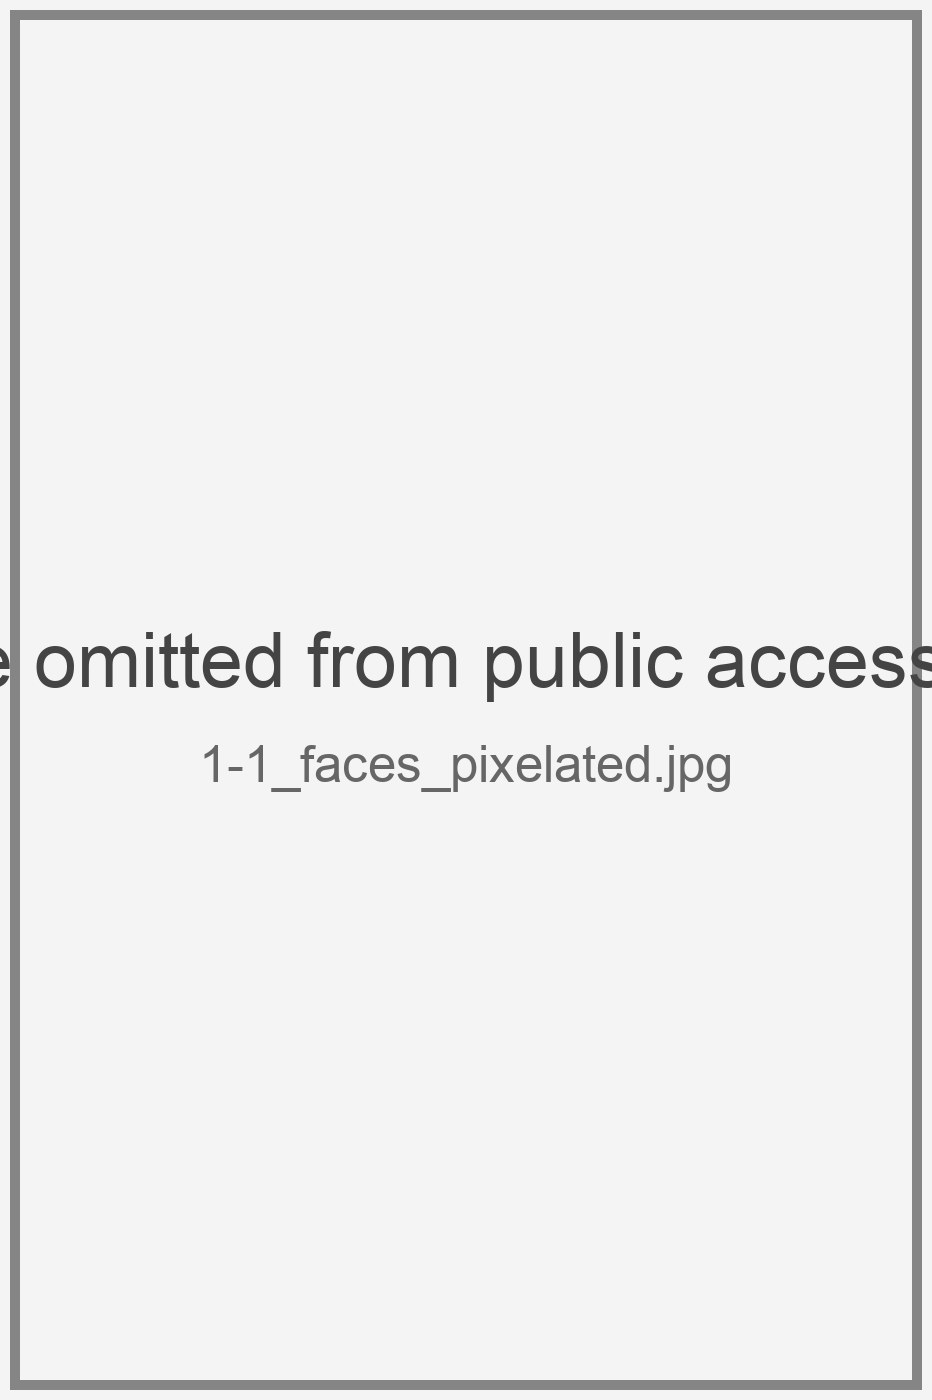
\includegraphics[width=\linewidth,height=0.18\textheight,keepaspectratio]
        {Figures/variant_cases/1-1_faces_pixelated.jpg}
        \caption{Faces pixelated.}
    \end{subfigure}
    \hfill
    \begin{subfigure}[t]{0.30\textwidth}
        \centering
        
\includegraphics[width=\linewidth,height=0.18\textheight,keepaspectratio]
        {Figures/variant_cases/1-1_contact_occluded.jpg}
        \caption{Contact region occluded.}
    \end{subfigure}

    \vspace{4mm}

    \begin{subfigure}[t]{0.46\textwidth}
        \centering
        
\includegraphics[width=\linewidth,height=0.15\textheight,keepaspectratio]
        {Figures/variant_cases/7-2_original.jpg}
        \caption{\texttt{7-2}: original.}
    \end{subfigure}
    \hfill
    \begin{subfigure}[t]{0.46\textwidth}
        \centering
        
\includegraphics[width=\linewidth,height=0.15\textheight,keepaspectratio]
        {Figures/variant_cases/7-2_pose_occluded.jpg}
        \caption{Body/pose occluded.}
    \end{subfigure}

    \vspace{4mm}

    \begin{subfigure}[t]{0.46\textwidth}
        \centering
        
\includegraphics[width=\linewidth,height=0.15\textheight,keepaspectratio]
        {Figures/variant_cases/12-1_original.jpg}
        \caption{\texttt{12-1}: original.}
    \end{subfigure}
    \hfill
    \begin{subfigure}[t]{0.46\textwidth}
        \centering
        
\includegraphics[width=\linewidth,height=0.15\textheight,keepaspectratio]
        {Figures/variant_cases/12-1_gestures_occluded.jpg}
        \caption{Hand/gesture region occluded.}
    \end{subfigure}

    \caption[Local-occlusion cases used in RQ4.]{Original and edited images for
    the local-occlusion cases used in RQ4. The corresponding output changes are
    reported in Table~\ref{tab:variant_transitions}.}
    \label{fig:app_local_edits}
\end{figure}

\clearpage

\begin{figure}[p]
    \centering

    \begin{subfigure}[t]{0.30\textwidth}
        \centering
        
\includegraphics[width=\linewidth,height=0.18\textheight,keepaspectratio]
        {Figures/variant_cases/16-1_original.jpg}
        \caption{\texttt{16-1}: original.}
    \end{subfigure}
    \hfill
    \begin{subfigure}[t]{0.30\textwidth}
        \centering
        
\includegraphics[width=\linewidth,height=0.18\textheight,keepaspectratio]
        {Figures/variant_cases/16-1_faces_occluded.jpg}
        \caption{Faces occluded.}
    \end{subfigure}
    \hfill
    \begin{subfigure}[t]{0.30\textwidth}
        \centering
        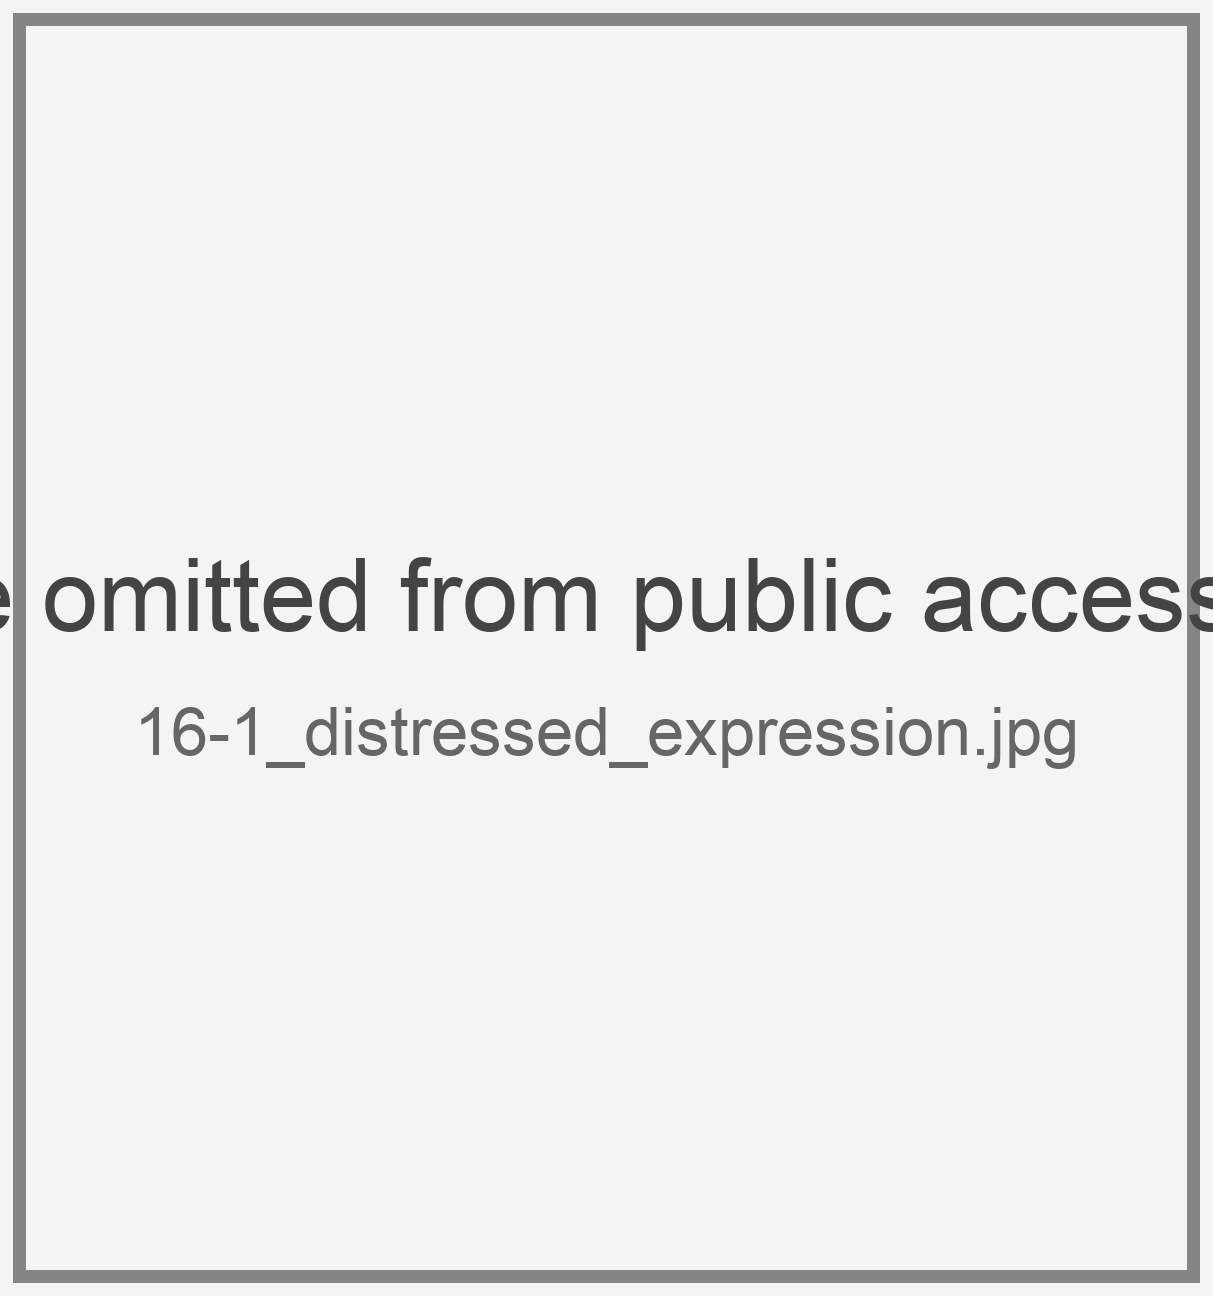
\includegraphics[width=\linewidth,height=0.18\textheight,keepaspectratio]
        {Figures/variant_cases/16-1_distressed_expression.jpg}
        \caption{Distressed expression.}
    \end{subfigure}

    \vspace{4mm}

    \begin{subfigure}[t]{0.30\textwidth}
        \centering
        
\includegraphics[width=\linewidth,height=0.18\textheight,keepaspectratio]
        {Figures/variant_cases/16-2_original.jpg}
        \caption{\texttt{16-2}: original.}
    \end{subfigure}
    \hfill
    \begin{subfigure}[t]{0.30\textwidth}
        \centering
        
\includegraphics[width=\linewidth,height=0.18\textheight,keepaspectratio]
        {Figures/variant_cases/16-2_faces_occluded.jpg}
        \caption{Faces occluded.}
    \end{subfigure}
    \hfill
    \begin{subfigure}[t]{0.30\textwidth}
        \centering
        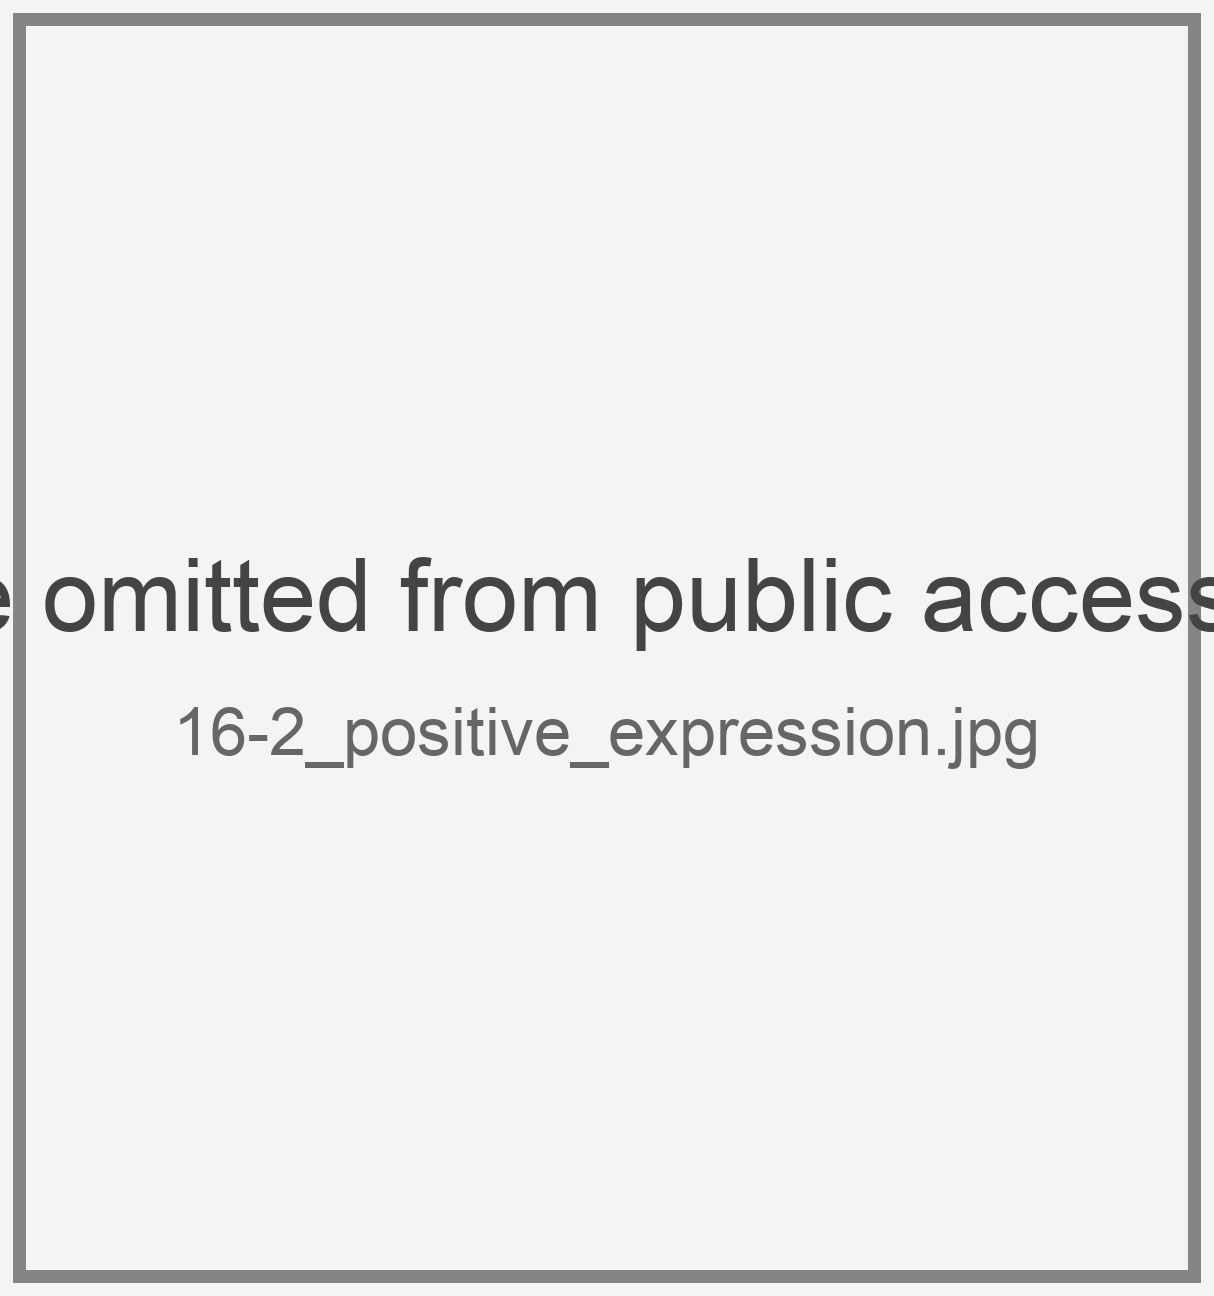
\includegraphics[width=\linewidth,height=0.18\textheight,keepaspectratio]
        {Figures/variant_cases/16-2_positive_expression.jpg}
        \caption{Positive expression.}
    \end{subfigure}

    \vspace{4mm}

    \begin{subfigure}[t]{0.43\textwidth}
        \centering
        
\includegraphics[width=\linewidth,height=0.18\textheight,keepaspectratio]
        {Figures/variant_cases/34-1_original.jpg}
        \caption{\texttt{34-1}: original.}
    \end{subfigure}
    \hfill
    \begin{subfigure}[t]{0.43\textwidth}
        \centering
        
\includegraphics[width=\linewidth,height=0.18\textheight,keepaspectratio]
        {Figures/variant_cases/34-1_text_removed.jpg}
        \caption{Readable text removed.}
    \end{subfigure}

    \caption[Facial-information and text-edit cases used in RQ4.]{Original and
    edited images used to examine facial information and embedded text in RQ4.}
    \label{fig:app_face_text_edits}
\end{figure}

\clearpage

\begin{figure}[p]
    \centering

    \begin{subfigure}[t]{0.46\textwidth}
        \centering
        
\includegraphics[width=\linewidth,height=0.20\textheight,keepaspectratio]
        {Figures/variant_cases/g-7_original.jpg}
        \caption{\texttt{g-7}: original.}
    \end{subfigure}
    \hfill
    \begin{subfigure}[t]{0.46\textwidth}
        \centering
        
\includegraphics[width=\linewidth,height=0.20\textheight,keepaspectratio]
        {Figures/variant_cases/g-7_group_occluded.jpg}
        \caption{Central group region occluded.}
    \end{subfigure}

    \vspace{6mm}

    \begin{subfigure}[t]{0.43\textwidth}
        \centering
        
\includegraphics[width=\linewidth,height=0.27\textheight,keepaspectratio]
        {Figures/variant_cases/32-2_original.jpg}
        \caption{\texttt{32-2}: disaster setting.}
    \end{subfigure}
    \hfill
    \begin{subfigure}[t]{0.43\textwidth}
        \centering
        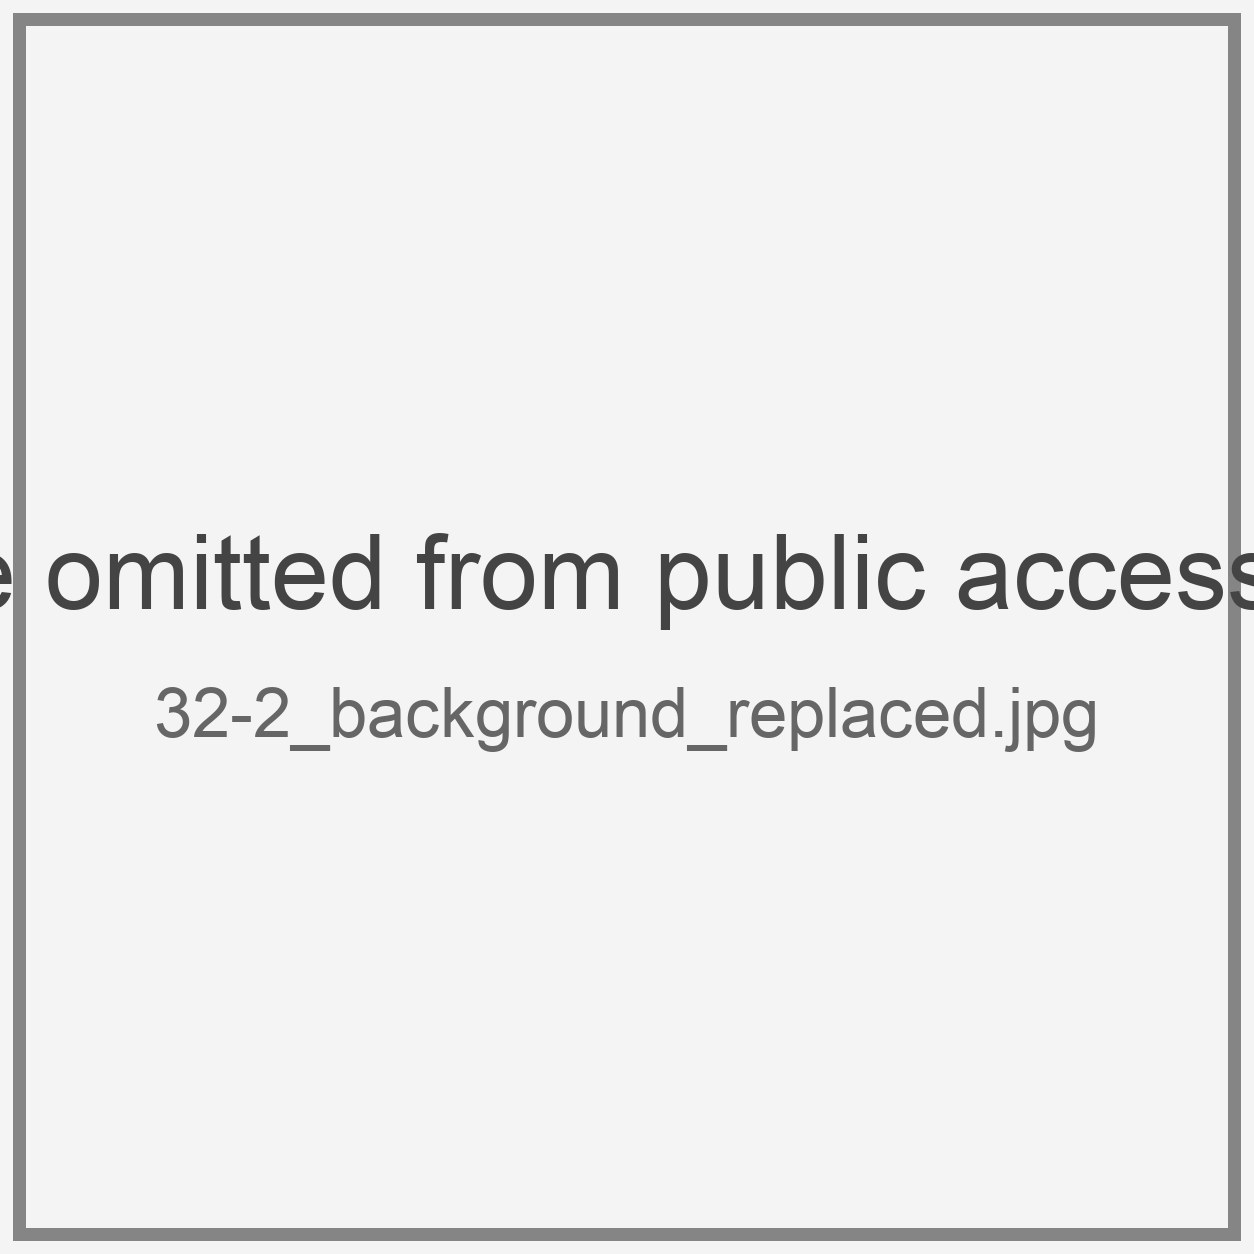
\includegraphics[width=\linewidth,height=0.27\textheight,keepaspectratio]
        {Figures/variant_cases/32-2_background_replaced.jpg}
        \caption{Peaceful replacement setting.}
    \end{subfigure}

    \caption[Group- and environmental-context edits used in RQ4.]{Original and
    edited images used to examine participant-group and environmental context
    in RQ4.}
    \label{fig:app_context_edits}
\end{figure}

\FloatBarrier